% --------------------------------------------------------------
% This is all preamble stuff that you don't have to worry about.
% Head down to where it says "Start here"
% --------------------------------------------------------------

\documentclass[12pt]{article}

\usepackage[margin=1in]{geometry}
\usepackage{amsmath,amsthm,amssymb}
\usepackage{graphicx}
\usepackage{subcaption}
\usepackage{algorithmicx}
\usepackage{algorithm}
\usepackage{algpseudocode}
\usepackage[colorlinks,linkcolor=blue]{hyperref}
\usepackage[noabbrev]{cleveref}
\usepackage{courier}
\usepackage{listings}
\usepackage{comment}


\oddsidemargin 0in
\evensidemargin 0in
\textwidth 6.5in
\topmargin -0.5in
\textheight 9.0in

\newcommand{\ignore}[1]{}
\def\pp{\par\noindent}

\newcommand{\assignment}[4]{
\thispagestyle{plain}
\newpage
\setcounter{page}{1}
\noindent
\begin{center}
\framebox{ \vbox{ \hbox to 6.28in
{CIS 419/519: Applied Machine Learning \hfill #1}
\vspace{4mm}
\hbox to 6.28in
{\hspace{2.5in}\large\bf\mbox{Homework #2}}
\vspace{4mm}
\hbox to 6.28in
{{\it Handed Out: #3 \hfill Due: #4}}
}}
\end{center}
}

\makeatletter
\renewcommand{\fnum@algorithm}{\fname@algorithm}
\makeatother

\lstset{basicstyle=\footnotesize\ttfamily,breaklines=true}
\lstset{framextopmargin=50pt,frame=bottomline}


\begin{document}

\assignment{Fall 2024}{2}{October 2}{7:59 pm October 22}

% --------------------------------------------------------------
%                         Start here
% --------------------------------------------------------------


{\bf Name: }  Alan Wu\\

{\bf PennKey:} alanlwu\\

{\bf PennID:} 41855518

\section{Declaration}
\begin{itemize}
\item \textbf{Person(s) discussed with:} \textit{Your answer}
\item \textbf{Affiliation to the course: student, TA, prof etc.} \textit{Your answer}
\item \textbf{Which question(s) in coding / written HW did you discuss?} \textbf{\textit{Your answer}}
\item \textbf{Briefly explain what was discussed.} \textit{Your answer}
\end{itemize}

\section{Multiple Choice \& Written Questions}

\begin{enumerate}
\item 
\begin{enumerate}
\item Our unregularized logistic regression decision boundary will probably be a line with some intercept (positive or negative) on the x1 or x2 axis. There will be 0-1 misclassified points. In our example, we have 2 misclassified points. Here is a simple example: \\ 

\begin{figure}[H]
  \centering
  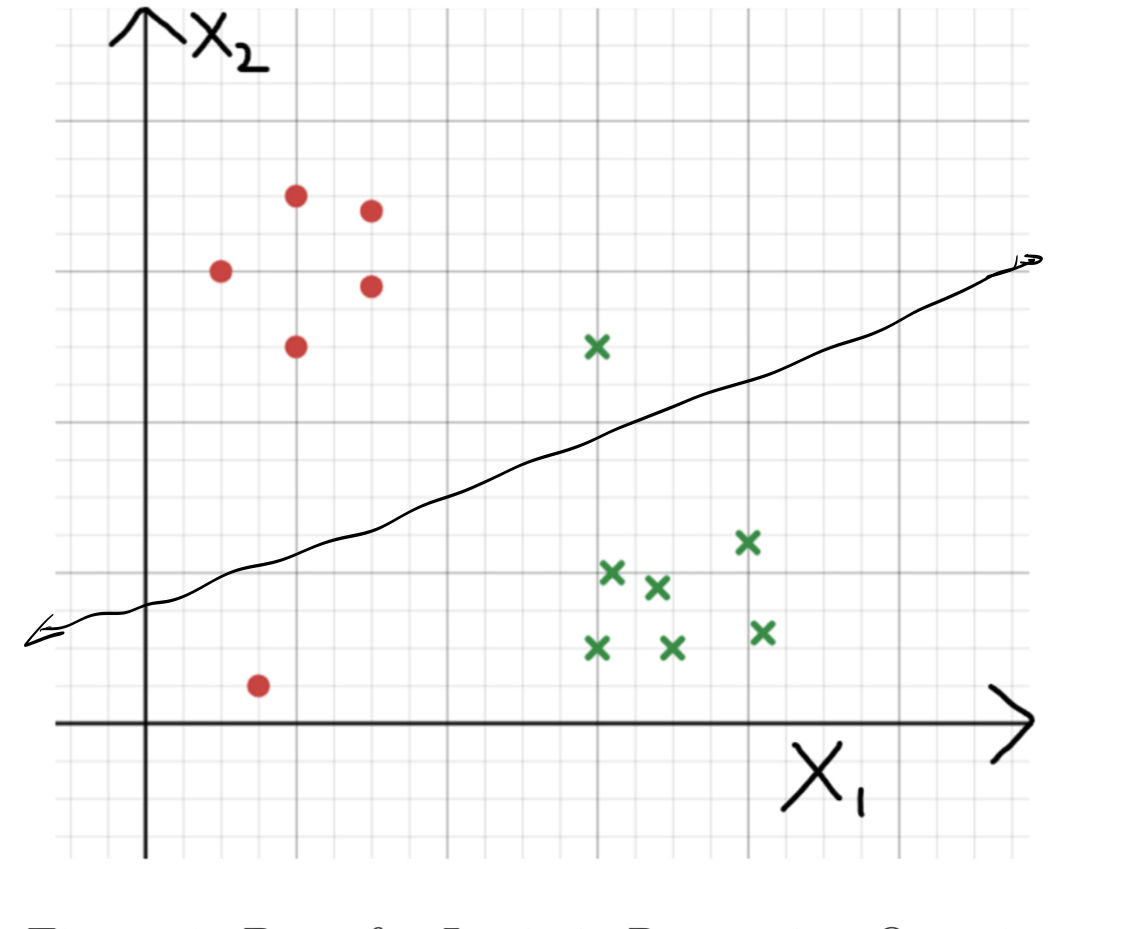
\includegraphics[width=0.5\textwidth]{1_a.jpeg}
  \caption{Unregularized Logistic Regression Decision Boundary}
\end{figure}
\item When we apply heavy regularization to the $\theta_0$ parameter, we can see that it will be pushed to 0. This means that the decision boundary will go through the origin, as when $x_1 = x_2$, the decision boundary will be 0 and the predicted probability of either class is 0.5. There should be 1-2 misclassified points. In our example, we have 1 misclassified point. And thus, our figure looks like this: \\ 
\begin{figure}[H]
  \centering
  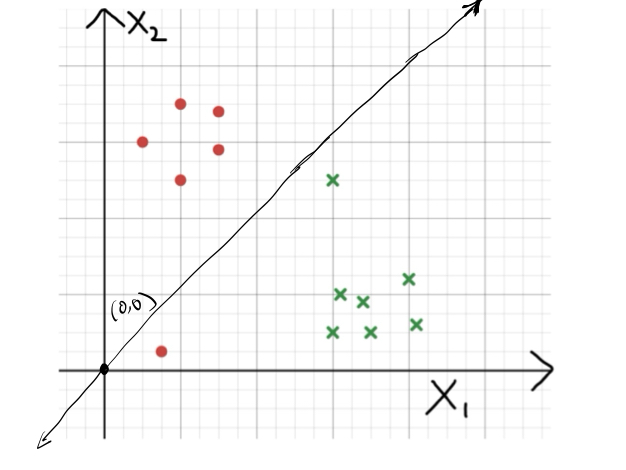
\includegraphics[width=0.5\textwidth]{1_b.jpeg}
  \caption{Heavy Regularized Logistic Regression on $\theta_0$ Decision Boundary}
\end{figure}
\item When we apply heavy regularization to the $\theta_1$ parameter, then that means that the $\theta_1$ parameter will be pushed to 0. Since we have the line as $\theta_0 + \theta_2 x_2$, then we know that we have the decision boundary $x_2 = -\theta_0/\theta_2$. Our decision boundary will be a horizontal line that splits the clusters into two on the $x_2$ axis. There should be 1-2 misclassifications. In our figure we have 2 misclassified points. Here is the figure: \\ 
\begin{figure}[H]
  \centering
  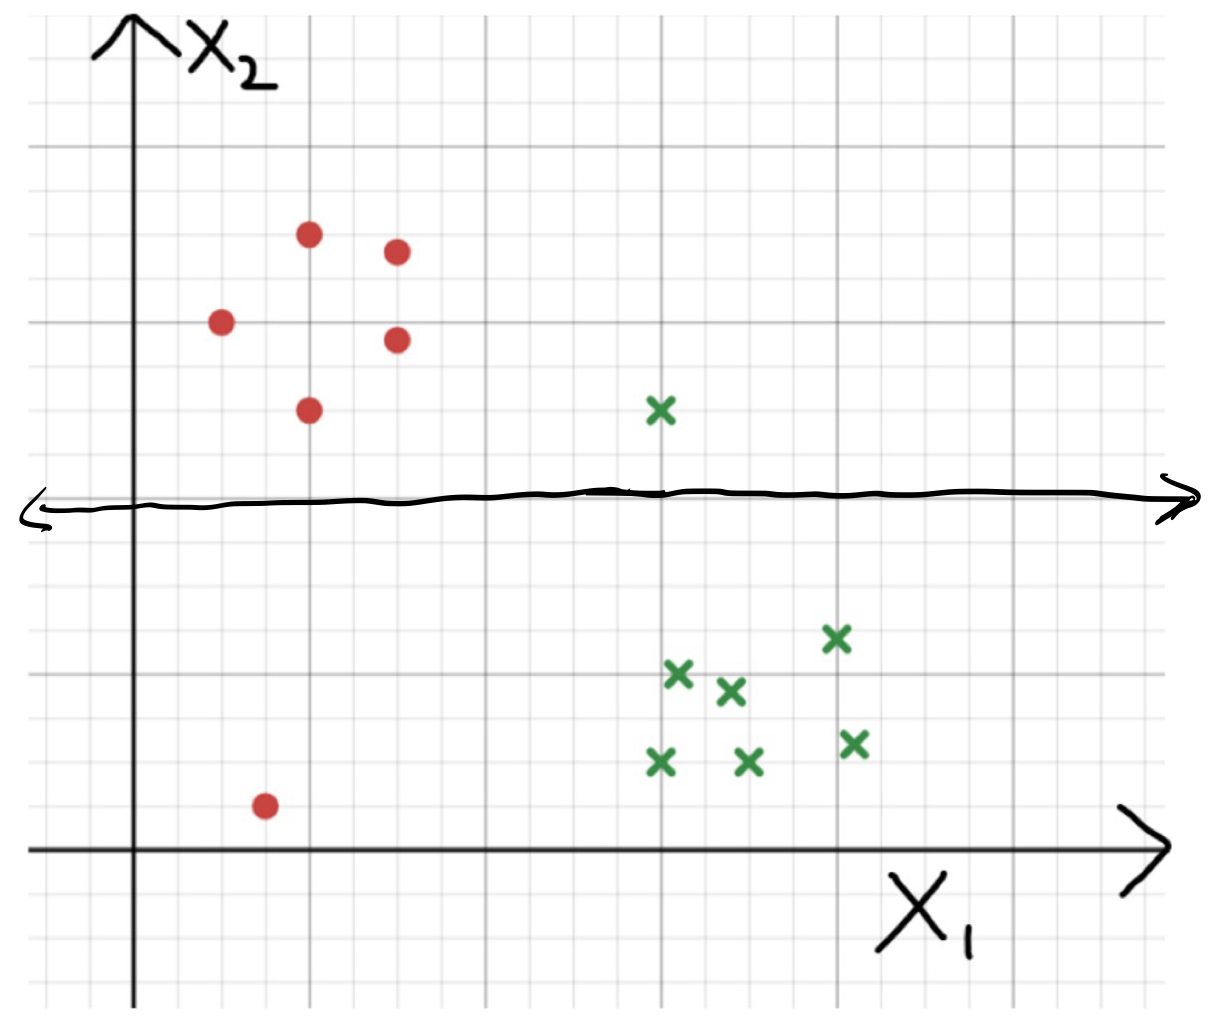
\includegraphics[width=0.5\textwidth]{1_c.jpeg}
  \caption{Heavy Regularized Logistic Regression on $\theta_1$ Decision Boundary}
\end{figure}
\item When we apply heavy regularization to the $\theta_2$ parameter, the $\theta_2$ parameter will be pushed to 0. In this case, our decision boundary will follow the line $\theta_0 + \theta_1 x_1$. Thus, the resulting decision boundary will be $x_1 = \theta_0 / \theta_1$, which will be a vertical line that runs through the $x_1$ axis. Our sample boundary has 0 misclassified points. Here is the figure: \\ 
\begin{figure}[H]
  \centering
  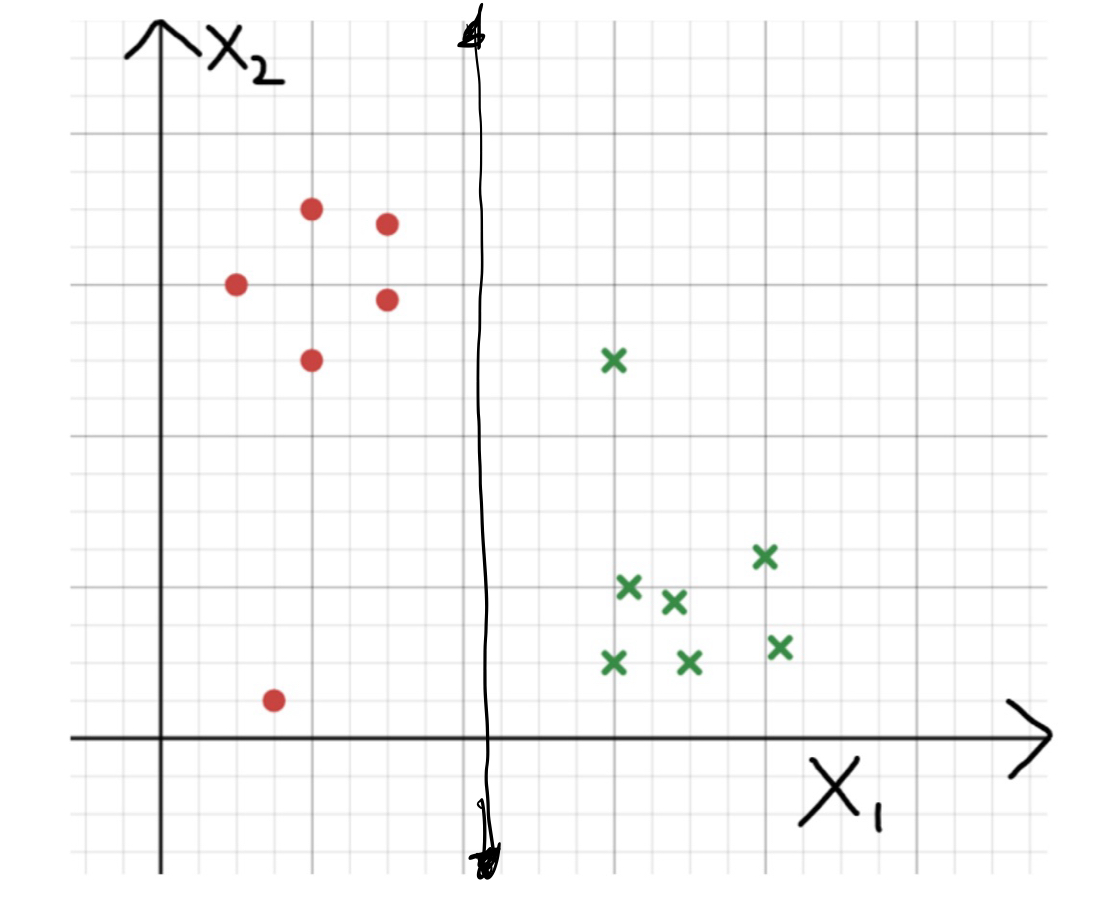
\includegraphics[width=0.5\textwidth]{1_d.jpeg}
  \caption{Heavy Regularized Logistic Regression on $\theta_2$ Decision Boundary}
\end{figure}
\end{enumerate}

\item
\begin{enumerate}
\item If we have two training points and we are using a k = 1 neighbors algorithm, then the decision boundary will be the line that is the perpendicular bisector of the midpoint of the two training points. We already know that k nearest neighbors algorithm will have decision boundary halfway through the two points because that point is equally distant from both points. Below details an example of this: \\ 
\begin{figure}[H]
  \centering
  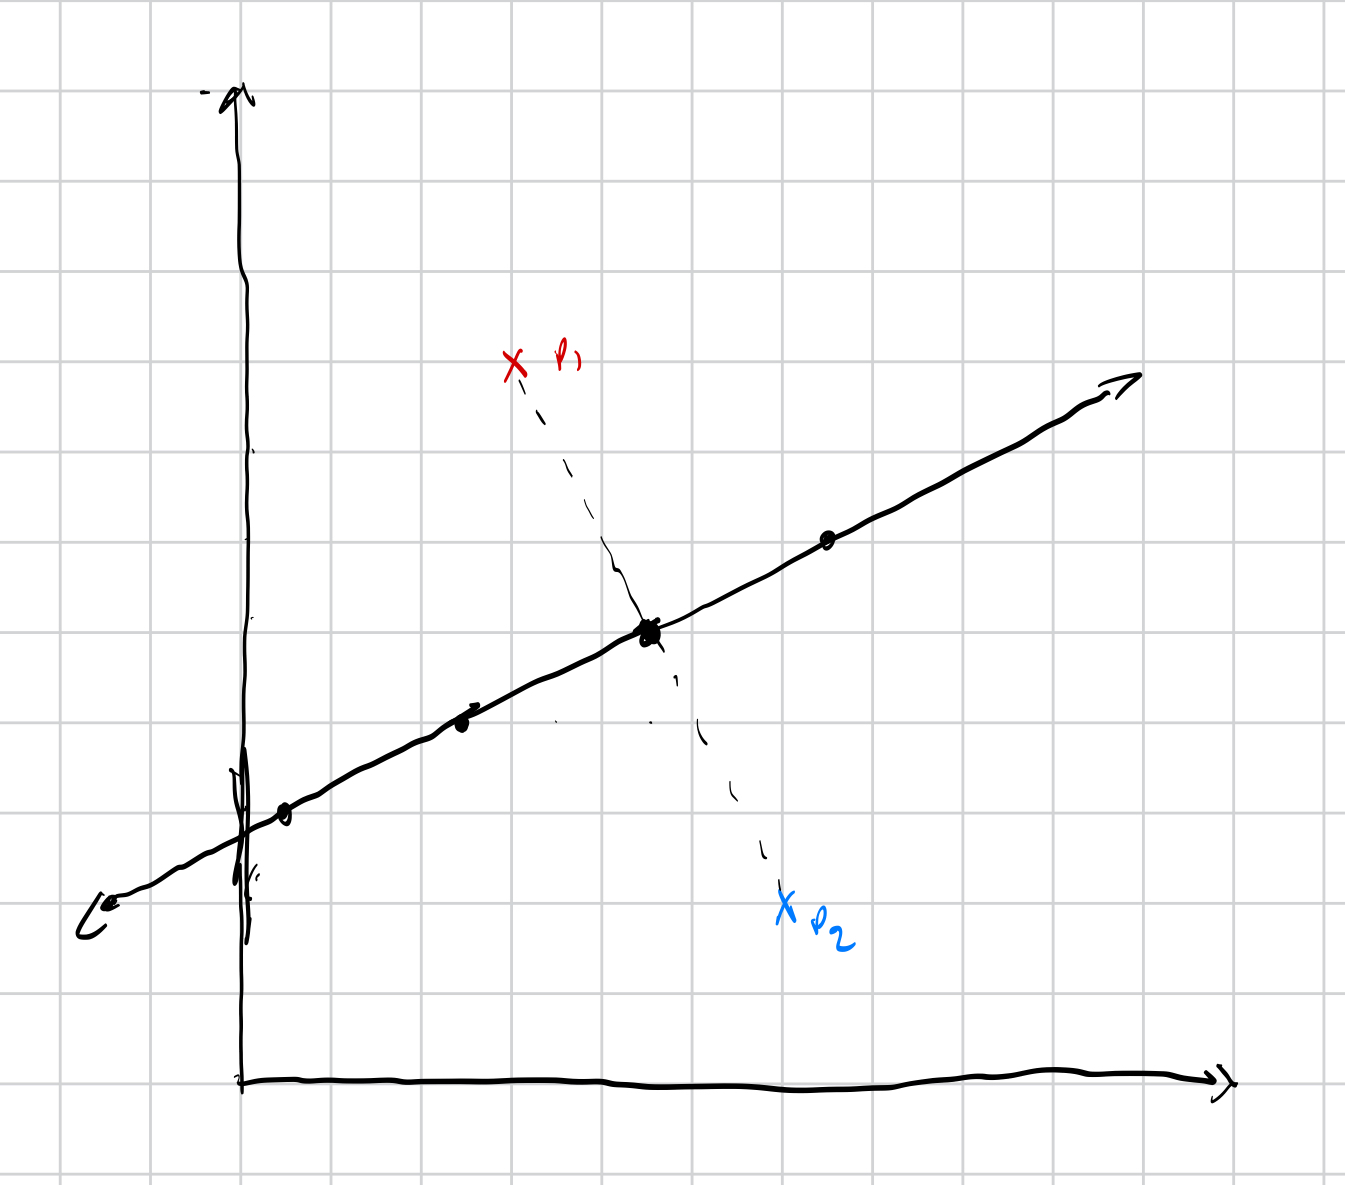
\includegraphics[width=0.5\textwidth]{2_a.jpeg}
  \caption{Decision Boundary K = 1}
  \label{fig:boundary}

\end{figure}
\item Yes, it can explain any dataset. It will be completely determined by the training data. 
\item As k approaches $\infty$, the decision boundary will become smoother. The resulting model function family will be the majority class of the training set, as when we use infinite point, we are essentially using the entire training set. 
\item Increasing the k will increase the bias and lower the variance. As we have more points to reference in our regression or classification, we will have a smoother decision boundary. Since there are a greater amount of points, the average of these points will be more representative of the true value of any given point. The bias increases because as we have more points, the average prediction will be closer to the true value. 
\item In KNN classification, we generally take the majority label and call it our prediction. We can adjust this for a given accuracy/recall/precision metric by simply changing how many values out of k we commit to a positive or negative class. Another approach we could use is to measure the probability of a given class by counting the number of positive and negative outcomes, and then determining the class prediction based on a threshold that we tune. 
\end{enumerate}

\item
  \begin{enumerate}
  \item We may expect that when we use post-pruning, we may not need early stopping. To clarify that this is indeed not the case, we can first consider what each of the concepts means and then see how they are related. Post pruning 
  occurs after we've finished building out the entire tree and then we begin to take out subsets of the tree and replace them as leaves if they do not improve the performance of the tree. We will keep pruning until taking away more tree subsets yields us negative validation set gains. On the other hand, early stopping will stop us from 
  building out the entire tree. This means that perhaps some features will not be split on or we will not have the full tree. In this way, it becomes clear why we could possibly need both. When we strictly use post-pruning, we are going to be post-pruning from a tree built out with all of its features. Given this fact, if some of the features are significantly not important, then we may still include them in the tree. We will prune the tree to a certain extent, but these features may already be overfitted to the noise in the training data. However, if we combine the early stopping and the post-pruning, we will start pruning with a tree that is well-fitted based on only the most significant features (as determined by ourselves) and then prune further to prevent our decision tree from overfitting.
  \item We are given the following conditions for when increasing the minimum samples needed to split will increase bias/variance: 
  
    \begin{enumerate}
      \item increase variance 
      \item increase bias 
      \item increase variance 
      \item increase variance
    \end{enumerate}

  \end{enumerate}

\item
  \begin{enumerate}
  \item We know the computation of the entropy of a given dataset is going to be $H(z) = -\sum_{y}P(Y=y)\log_2 P(Y=y)$
  
  Therefore, we can compute the entropy of the dataset as follows: \\ 

  There are 3 positive samples and 1 negative sample thus  

    \begin{align}
      H(z) = -\sum_y{P(Y=y)\log_2 P(y=y)} \notag \\ 
      = -[P(Y=1)\log_2 P(Y=1) + P(Y=0)\log_2 P(Y=0)] \notag \\ 
      = -[0.75 \log_2 (0.75) + 0.25 \log_2 (0.25)] \notag \\ 
      = 0.811 \notag
    \end{align}

    Therefore, the entropy of the current training samples is 0.811.

  \item The information gain is going to be the entropy of the parent node minus the weighted sum of the entropy of the child nodes. We will have to first define the computation for each of the features a1 and a2: \\ 
  
  $IG(Z, a1) = H(Z) - H(Z[a1 = 1])P(a1 = 1) - H(Z[a1=0])P(a1=0)$ and \\ 

  $IG(Z, a2) = H(Z) - H(Z[a2 = 1])P(a2 = 1) - H(Z[a2=0])P(a2=0)$ \\ 

  We will compute the individual information gain for each of the features, first for a1. We will use that there are 2 samples where feature a1 is positive and 2 where a1 is negative. Of all the samples for a1, 1 of them is negative and 3 samples are positive.

  \begin{align*}
   & IG(Z, a1) = H(Z) - H(Z[a1=1])P(a1=1) - H(Z[a1=0])P(a1=0)  \notag \\ 
   & = 0.811 + [P(Y=1|a1=1)\log_2 P(Y=1|a1=1) \notag \\ 
   & + P(Y=0|a1=1)\log_2 P(Y=0|a1=1)]P(a1=1) + \notag \\ 
   & [P(Y=1|a1=0)\log_2P(Y=1|a1=0) + P(Y=0|a1=0)\log_2P(Y=0|a1=0)]P(a1=0) \notag \\ 
   & = 0.811 + [1 \log_2 1 + 0 \log_2 0] 0.5 + [0.5 \log_2 0.5 + 0.5 \log_2 0.5] 0.5 \notag \\ 
   & = 0.811 - log_2 0.5 \notag \\ 
   & = 0.311 \notag
  \end{align*}
  
  The information gain of the dataset with respect to feature a1 is 0.311. \\ 

  Let's compute the individual information gain for a2: Note that for a2, there are 3 samples where feature a2 is positive and 1 sample where a2 is negative (with respect to itself). Of all the samples for a2, 3 of them are classified as positive and 1 of them is classified as negative. 

  \begin{align*}
    & IG(Z, a2) = H(Z) - H(Z[a2=1])P(a2=1) - H(Z[a2=0])P(a2=0)  \notag \\ 
    & = 0.811 + [P(Y=1|a2=1)\log_2 P(Y=1|a2=1) \notag \\ 
    & + P(Y=0|a2=1)\log_2 P(Y=0|a2=1)]P(a2=1) + \notag \\ 
    & = 0.811 + [0.667 \log_2 0.667 + 0.333 \log_2 0.333] 0.75 + [1 \log_2 1 + 0] 0.25 \notag \\ 
    & = 0.811 - (0.918) * 0.75 \notag \\ 
    & = 0.811 - 0.689 \notag \\ 
    & = 0.122 \notag
  \end{align*}

  The information gain of the dataset with respect to feature a2 is 0.122.

  \item The figure:  \\ 
  
  \begin{figure}[H]
    \centering
    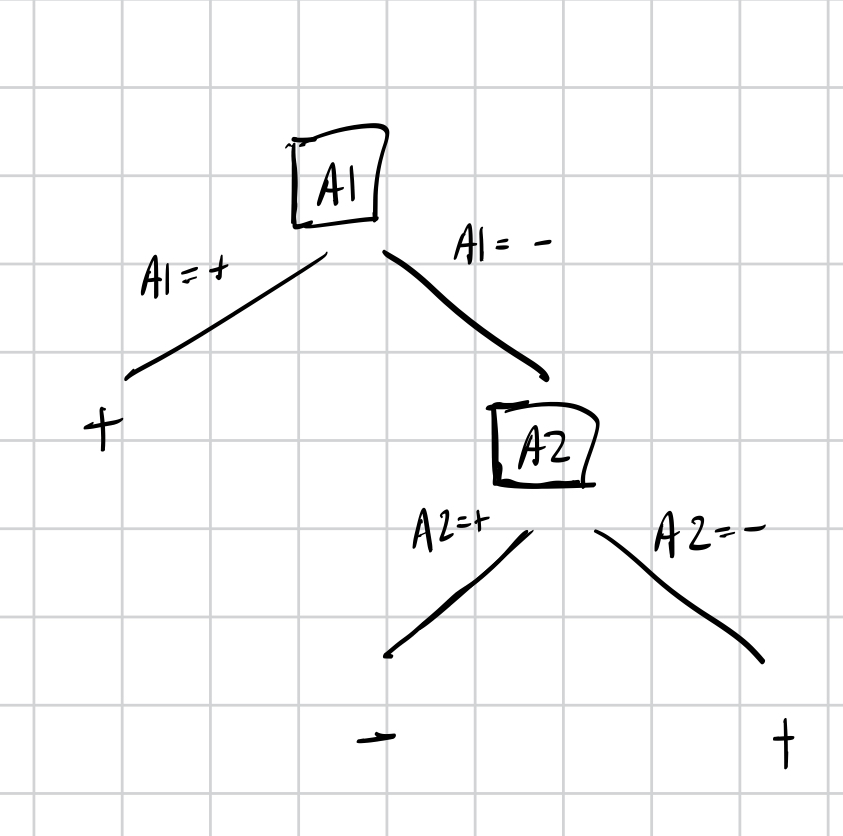
\includegraphics[width=0.5\textwidth]{3_c.jpeg}
    \caption{Decision Tree}
    \label{fig:tree}
  \end{figure}



  \end{enumerate}
 \item
 \begin{enumerate}
     \item K Nearest Neighbors algorithm assumes that the predictions will be close in some arbitrary distance function. In this way, for our problem, since we are trying to predict the binary outcome of a house price, then we are assuming that houses that have similar prices are similar in square footage and also the number of bedrooms.
     \item Euclidean distance will be a bad metric given our two features: square footage and the number of bedrooms because the two features are not on the same scale. The number of bedrooms is a discrete variable that takes on low values of 1, 2, 3, etc. while the square footage of the house is a continuous variable that can take on any value, usually in the thousands. If we use the variables as they are, the square footage will dominate the distance computation. What we can do to solve the issue is normalize both variables on the same scale (say on the z-score scale or limit it to 0 to 1).
     \item The type of roof a house has would not be a good feature for our model. The two other features are numerical features where the numerical value of the feature takes on some important. This is not the case for the type of roof, as the numerical value simply represents a category. 
     \item The training complexity is $O(N * D)$, where $N$ is the number of training samples and $D$ is the number of features. We will have to go through all $N$ training samples to find the nearest neighbor. We will also have to go through all $D$ features to compute the distance between the test sample and the training sample.
     \item The curse of dimensionality is a concept where once our training data has many many features, the distance between the nearest and the farthest neighbors becomes very similar. As the number of dimensions increases, the volume of the space increases exponentially. This becomes a problem because our nearest neighbors are not going to be very predictive of the test sample (s).
 \end{enumerate}

 \item 
 \begin{enumerate}
      \item True 
      \item immediately before the last sigmoid activation function
      \item $2K^2$
      \item True
      \item False
 \end{enumerate}

\end{enumerate}

\section{Python Programming Questions}

% Complete questions in your iPython notebook and place all results here.

\begin{itemize} 
  \item \textbf{Question 1: }
  \item \textbf{Question 2: }
  \item \textbf{Question 3: }
  \item \textbf{Question 4: }
  \item \textbf{Question 6: }
\end{itemize}

\end{document} 